\chapter{Oxygen}
\label{chap:o2}
\section{Recent developments}
    \Abinitio{} studies for the ${\rm O_2 - O_2}$ system are computationally difficult due to the open shell nature of the monomer $\rm{O_2}$ which prevents the orthogonalization of the monomer wavefunctions \cite{Bussery1993}. Recently it is gaining popularity in the field of buffer gas cooling and trapping of oxygen \cite{Friedrich1998,Avdeenkov2001}. Since the ground state monomer exists in the triplet state, there are three possible molecular spin states (denoted as singlet, triplet and quintet) and associated \PESs{}. The short-range exchange interactions were known to cause not only repulsion but also splitting between the molecular spin states of the dimer. Computationally expensive short-range exchange calculations using the Heisenberg Hamiltonian were first performed by van Hemert et al. \cite{vanHemert1983} in a preliminary study and later by Wormer and van der Avoird \cite{Wormer1984}. The authors reported \abinitio{} calculations including electrostatic as well as exchange interactions but excluding long range dispersion interactions as they were primarily interested in studying the solid phase magnetic properties of the dimer. They reported \PESs{} for the three different spin states using spherical expansion to represent the orientational dependence and exponential functions to represent the dependence on intermolecular distance.  By including first order electrostatic and exchange contributions \abinitio{}, second order polarization energy semi-empirically, Bussery and Wormer \cite{Bussery1993} reported improved \PESs{} for the oxygen dimer and used it mainly for studying optical properties. By accounting for dipole-dipole as well as multipole-multipole contributions, they were able to accurately capture the intermolecular correlation energy. The simple analytic form of the polarization energy helped improve their overall computational efficiency as well. The gas phase second virial coefficients computed using the different \PESs{} were found to be in very good statistical agreement with experiments. Really precise molecular beam experiments were performed by Aquilanti et al. \cite{Aquilanti1999} to obtain anisotropic \PESs{} using a spherical harmonics expansion but including only four terms. This led to a simplified potential model with less number of fitted parameters. Upon comparison with the \abinitio{} calculations of Bussery et al. \cite{Bussery1993}, they found good agreement for various geometrical predictions related to the dimer structure. Hernández-Lamoneda et al. \cite{Lamoneda2005CPL} in a preliminary study and later Bartolomei et al. \cite{Bartolomei2008} performed really accurate \abinitio{} calculations at RCCSD(T) level of theory for the quintet state of the oxygen dimer. This was possible only for the quintet state because of the acceptable nature of a single configuration reference as the zeroth-order function. Such highly accurate calculations are not possible for the singlet and triplet states. However, MRCI calculations, albeit with size inconsistency issues can still be applied to study these states. By accurately extracting the spin-coupling parameter $J$ involved in the Heisenberg Hamiltonian within the MRCI calculations and combining it with accurate spin-averaged interaction potential from the RCCSD(T) calculations, they were able to obtain high quality \PESs{} than previous studies. Zuchowski \cite{Zuchowski2008} performed SAPT based DFT calculations for the quintet state and observed very good agreement with previous accurate \abinitio{} coupled-cluster calculations. More recently Bartolomei et al. \cite{Bartolomei2010} have obtained completely \abinitio{} \PESs{} for the three spin states by combining their previous RCCSD(T) data \cite{Bartolomei2008} for the quintet state with new \abinitio{} calculations at the CASPT2 and MRCI levels of theory for the singlet and triplet states. By including dynamical electron correlation at higher levels of theory than previous calculations, they were able to improve the accuracy of the \PESs{}. They observed very good agreement with experiments for their second virial coefficients as well as integral cross sections.
\section{Computational details}
    The \abinitio{} potentials for the different spin multiplicities (s = 0, 1 and 2) and using different levels of theory i.e. MRCI and PT2 were due to Bartolomei et al. \cite{Bartolomei2010}. As we can see, we have 6 different potential surfaces that were reported. The full dimer virial coefficients are obtained for each level of theory by combining the individual spin virial coefficient value according to the formula \cite{Aquilanti1999,Bartolomei2010}:
    \begin{equation}
        \label{eq:o2combination}
        B_2 = \frac{B_2^0 + 3 B_2^1 + 5 B_2^2}{9}.
    \end{equation}
    where $B_2^s$ represents the second virial coefficient value computed using the appropriate potential based on the level of theory and the spin multiplicity $s$.

    We have performed classical and PIMC virial coefficient simulations at both levels of theory, all the spin multiplicities and set of 15 temperatures reported. For each type of classical simulation, we have collected $10^8$ configuration samples that were generated using two types of MC trials 1) translation and 2) rotation of the dimer. The PIMC simulations involved $P$ = 8, 16, 32 and 64 images for each condition mentioned above and we collected $10^7$ configuration samples per PIMC simulation. Apart from the translation of the dimer, we also include MC trials to regrow the ring by translating the beads (see Sec. \ref{subsec:orMove}) and our recently developed orientation algorithm \cite{hydrogen} (explained in Sec. \ref{subsec:orMove}).

    To avoid nonphysical values of the intermolecular energy for oxygen dimers, an artificial hard core with a diameter of 4.5 Bohr was used in all virial coefficient calculations. All the oxygen MSMC simulations involved a Hard Sphere reference with a diameter of 4.5 \AA.
\section{Results and discussion}
    We have computed classical as well as quantum virial coefficients using PIMC with $P$ = 8, 16, 32 and 64 images for both the MRCI and the PT2 \PESs{}. In general, our classical and PIMC results agree well with those of Bartolomei et al. \cite{Bartolomei2010} for the range of temperatures considered. In Fig. \ref{fig:B2O2AllExpDiffMRCI} we plot the difference between various second virial coefficient values calculated using the MRCI \PESs{} and experimental results, as a function of temperature.
    \begin{figure}[!htbp]
        \centering
        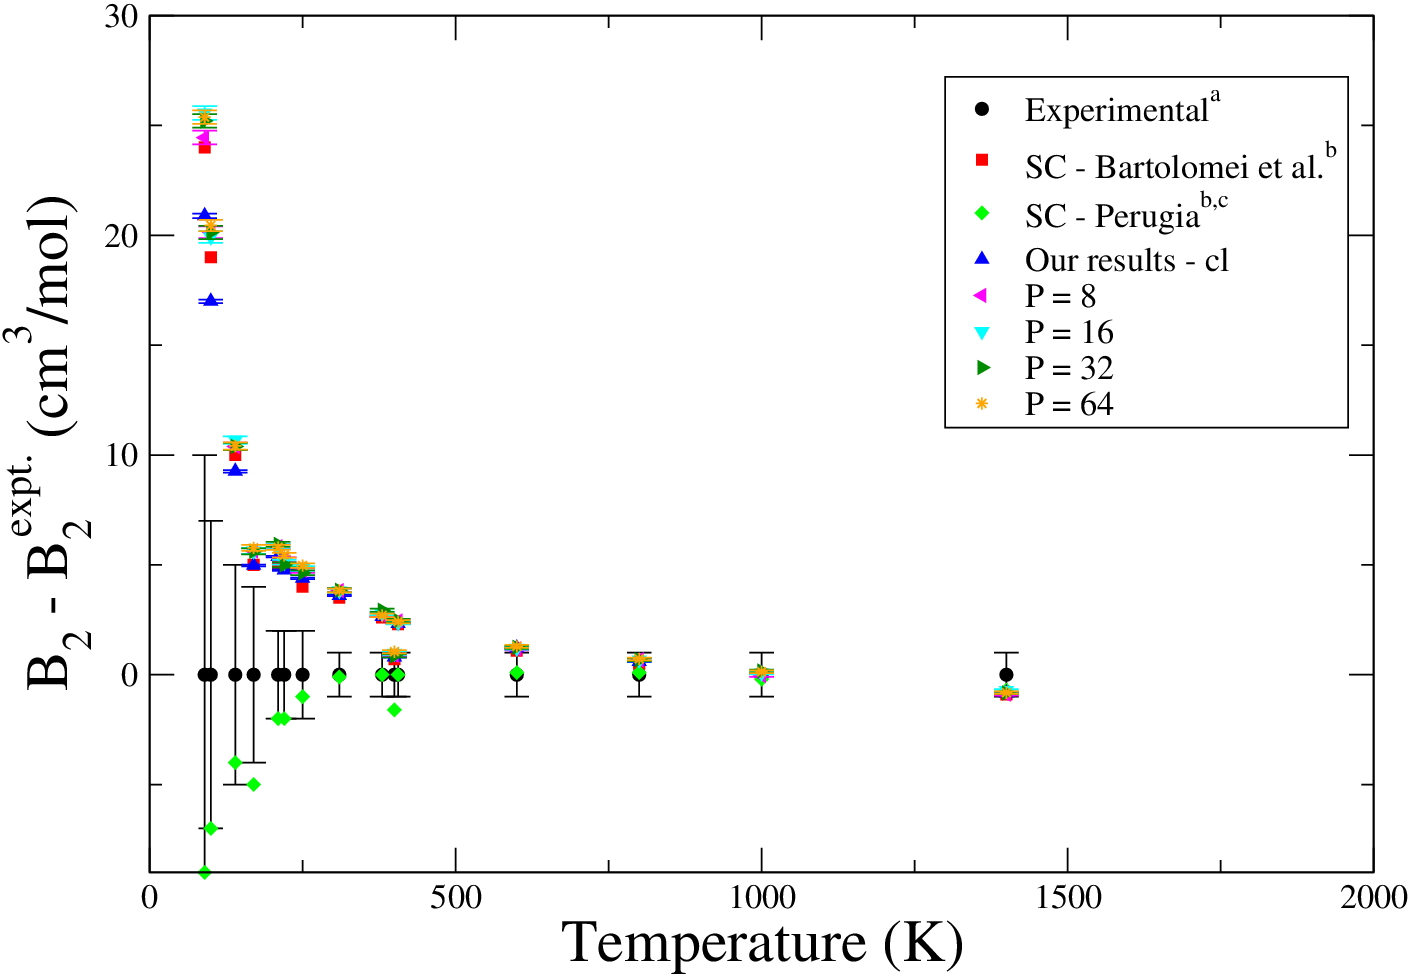
\includegraphics[scale=0.20,keepaspectratio]{Chapter-6/Figures/B2O2AllExpDiffMRCI.png}
        \caption{Difference between various second virial coefficient ($B_2$) values of oxygen computed using the MRCI \PESs{} and experimental results reported in Refs. \cite{Bartolomei2010,Dymond}. SC - MRCI and SC - Perugia represent semi-classical results of Bartolomei et al. \cite{Bartolomei2010} by using the MRCI and Perugia \PESs{} \cite{Aquilanti1999} respectively; CL - MRCI and PI - MRCI are our classical and PIMC results respectively.}
        \label{fig:B2O2AllExpDiffMRCI}
    \end{figure}

    From Fig. \ref{fig:B2O2AllExpDiffMRCI}, it can be seen that the semi-classical MRCI calculations performed by Bartolomei et al. \cite{Bartolomei2010} agrees with our PIMC calculations for the same \PESs{}, better than other semi-classical or classical calculations. We observe significant deviations from the experimental results even at temperatures as high as 400K. This can be attributed to the quality of the MRCI potential. We note that Bartolomei et al. \cite{Bartolomei2010} achieved better agreement with experiments after modifying isotropic parameters of the spherical harmonic function to match those of the Perugia group \cite{Aquilanti1999}. These modified parameters were however, not used by us and hence, the cause of such large deviations at temperatures lower than 400K. Also, we observe that our classical results using the MRCI \PESs{} start to deviate from our corresponding $P$ = 64 results using PIMC for temperatures $T \le 200$K and the semi-classical results of Bartolomei et al. \cite{Bartolomei2010} agree well with all our PIMC results for the temperatures $T > 250$K. This suggests quantum effects are well accounted for by the semi-classical calculations using the MRCI \PESs{} for $T > 200$K and we need to investigate lower temperatures in order to notice a significant difference between the semi-classical treatment and PIMC method.

    In Fig. \ref{fig:B2O2AllExpDiffPT2} we plot the difference between various second virial coefficient values calculated using the PT2 \PESs{} and experimental results, as a function of temperature.
    \begin{figure}[!htbp]
        \centering
        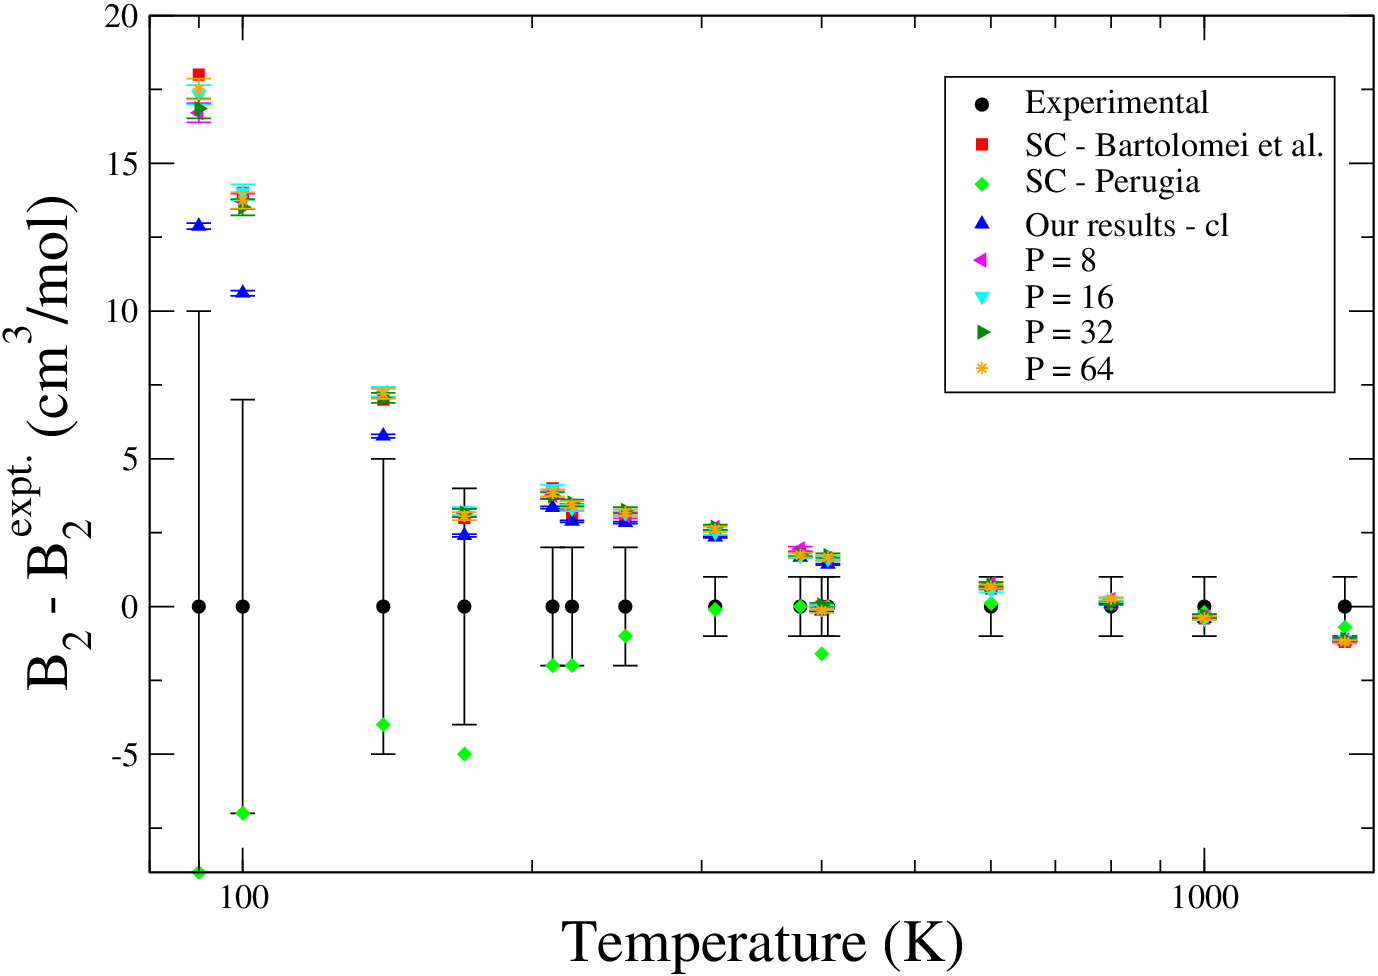
\includegraphics[scale=0.20,keepaspectratio]{Chapter-6/Figures/B2O2AllExpDiffPT2.png}
        \caption{Difference between various second virial coefficient ($B_2$) values of oxygen computed using the PT2 \PESs{} and experimental results reported in Refs. \cite{Bartolomei2010,Dymond}. SC - PT2 and SC - Perugia represent the semi-classical results of Bartolomei et al. \cite{Bartolomei2010} by using the PT2 and Perugia \PESs{} \cite{Aquilanti1999} respectively; CL - PT2 and PI - PT2 are our classical and PIMC results respectively.}
        \label{fig:B2O2AllExpDiffPT2}
    \end{figure}

    From Fig. \ref{fig:B2O2AllExpDiffPT2}, we observe a trend very similar to that of Fig. \ref{fig:B2O2AllExpDiffMRCI}. Here too, it can be seen that the semi-classical PT2 calculations performed by Bartolomei et al. \cite{Bartolomei2010} agrees with our PIMC calculations for the same \PESs{}, better than other semi-classical or classical calculations. The deviations observed from experimental results can be explained by the achievement of better agreement by Bartolomei et al. \cite{Bartolomei2010} with experiments upon modification of certain terms of their PT2 \PESs{}. Also, we observe that our classical results using the PT2 \PESs{} start to deviate from our corresponding $P$ = 64 results using PIMC for temperatures $T \le 275$K and the semi-classical results of Bartolomei et al. \cite{Bartolomei2010} agree with all our PIMC results for the temperatures considered. This suggests quantum effects are well accounted for by the semi-classical calculations using the PT2 \PESs{} for the temperatures considered and we need to investigate lower temperatures in order to notice a significant difference between the semi-classical treatment and PIMC method. We note that the agreement of the Perugia PES is consistently better than the MRCI or PT2 \PESs{}. This suggests that we might achieve more accurate results by the use of the Perugia \cite{Aquilanti1999} PES.

    \section{Conclusions}
        We have calculated fully quantum second virial coefficients for the oxygen dimer based on recent \abinitio{} \PESs{} due to Bartolomei et al. \cite{Bartolomei2010}. We have implemented the orientation sampling algorithm that was recently developed \cite{hydrogen} in PIMC calculations. We observed good agreement with most accurate semi-classical values available in literature. These results add further confidence on the capabilities of the algorithm in combination with PIMC to predict accurate quantum virial coefficients. The agreement with experimental results was found to be poor for PIMC results using both the MRCI and PT2 \PESs{}. This was attributed to inaccuracies in the reported \PESs{}. Quantum effects were found to be significant for $T \le 200$K using the MRCI potential whereas the semi-classical calculations of Bartolomei et al. \cite{Bartolomei2010} using the PT2 \PESs{} were found to be sufficient for all temperatures considered.

    \section{Tabulated Results}
    \label{sec:chap6-tables}
        We report tabulated results for the virial coefficients of oxygen in this section.
        \pgfplotstableset{
            begin table=\begin{longtable},
            end table=\end{longtable},
        }
        \pgfplotstabletypeset[
            columns/temperature/.style={
                string type,
                column name={Temperature(\si{\kelvin})}
            },
            columns/b2cb0/.style={
                string type,
                column name=B$^{0}_2$(\si{cm^3/mol})
            },
            columns/b2cb1/.style={
                string type,
                column name=B$^{1}_2$(\si{cm^3/mol})
            },
            columns/b2cb2/.style={
                string type,
                column name=B$^{2}_2$(\si{cm^3/mol})
            },
            columns/b2cbtot/.style={
                string type,
                column name=B$_2$(\si{cm^3/mol})
            },
            every head row/.append style={before row={\caption{Second virial coefficient of oxygen as a function of temperature using PIMC method with $P$ = 8 and MRCI potential of Bartolomei et al.\cite{Bartolomei2010}. Here B$^s_2$ represents the second virial coefficients evaluated using MRCI potential with multiplicity $s$. B$_2$ represents the final value obtained according to Eq. \eqref{eq:o2combination}. Values in parantheses are standard uncertainties in the rightmost digit(s).}\label{tab:7s8nbMRCIpotPIResults}\\\toprule},after row=\midrule\endfirsthead},
            every first row/.append style={before row={\multicolumn{5}{c}{\tablename\ \thetable{} -- Continued from previous page.}\\\toprule},after row=\midrule\endhead},
            every last row/.style={after row=\bottomrule},
        ]{Chapter-6/Tables/7s8nbMRCIpotPIResultsTable.dat}

        \pgfplotstabletypeset[
            columns/temperature/.style={
                string type,
                column name={Temperature(\si{\kelvin})}
            },
            columns/b2cb0/.style={
                string type,
                column name=B$^{0}_2$(\si{cm^3/mol})
            },
            columns/b2cb1/.style={
                string type,
                column name=B$^{1}_2$(\si{cm^3/mol})
            },
            columns/b2cb2/.style={
                string type,
                column name=B$^{2}_2$(\si{cm^3/mol})
            },
            columns/b2cbtot/.style={
                string type,
                column name=B$_2$(\si{cm^3/mol})
            },
            every head row/.append style={before row={\caption{Second virial coefficient of oxygen as a function of temperature using PIMC method with $P$ = 16 and MRCI potential of Bartolomei et al.\cite{Bartolomei2010}. Here B$^s_2$ represents the second virial coefficients evaluated using MRCI potential with multiplicity $s$. B$_2$ represents the final value obtained according to Eq. \eqref{eq:o2combination}. Values in parantheses are standard uncertainties in the rightmost digit(s).}\label{tab:7s16nbMRCIpotPIResults}\\\toprule},after row=\midrule\endfirsthead},
            every first row/.append style={before row={\multicolumn{5}{c}{\tablename\ \thetable{} -- Continued from previous page.}\\\toprule},after row=\midrule\endhead},
            every last row/.style={after row=\bottomrule},
        ]{Chapter-6/Tables/7s16nbMRCIpotPIResultsTable.dat}

        \pgfplotstabletypeset[
            columns/temperature/.style={
                string type,
                column name={Temperature(\si{\kelvin})}
            },
            columns/b2cb0/.style={
                string type,
                column name=B$^{0}_2$(\si{cm^3/mol})
            },
            columns/b2cb1/.style={
                string type,
                column name=B$^{1}_2$(\si{cm^3/mol})
            },
            columns/b2cb2/.style={
                string type,
                column name=B$^{2}_2$(\si{cm^3/mol})
            },
            columns/b2cbtot/.style={
                string type,
                column name=B$_2$(\si{cm^3/mol})
            },
            every head row/.append style={before row={\caption{Second virial coefficient of oxygen as a function of temperature using PIMC method with $P$ = 32 and MRCI potential of Bartolomei et al.\cite{Bartolomei2010}. Here B$^s_2$ represents the second virial coefficients evaluated using MRCI potential with multiplicity $s$. B$_2$ represents the final value obtained according to Eq. \eqref{eq:o2combination}. Values in parantheses are standard uncertainties in the rightmost digit(s).}\label{tab:7s32nbMRCIpotPIResults}\\\toprule},after row=\midrule\endfirsthead},
            every first row/.append style={before row={\multicolumn{5}{c}{\tablename\ \thetable{} -- Continued from previous page.}\\\toprule},after row=\midrule\endhead},
            every last row/.style={after row=\bottomrule},
        ]{Chapter-6/Tables/7s32nbMRCIpotPIResultsTable.dat}

        \pgfplotstabletypeset[
            columns/temperature/.style={
                string type,
                column name={Temperature(\si{\kelvin})}
            },
            columns/b2cb0/.style={
                string type,
                column name=B$^{0}_2$(\si{cm^3/mol})
            },
            columns/b2cb1/.style={
                string type,
                column name=B$^{1}_2$(\si{cm^3/mol})
            },
            columns/b2cb2/.style={
                string type,
                column name=B$^{2}_2$(\si{cm^3/mol})
            },
            columns/b2cbtot/.style={
                string type,
                column name=B$_2$(\si{cm^3/mol})
            },
            every head row/.append style={before row={\caption{Second virial coefficient of oxygen as a function of temperature using PIMC method with $P$ = 64 and MRCI potential of Bartolomei et al.\cite{Bartolomei2010}. Here B$^s_2$ represents the second virial coefficients evaluated using MRCI potential with multiplicity $s$. B$_2$ represents the final value obtained according to Eq. \eqref{eq:o2combination}. Values in parantheses are standard uncertainties in the rightmost digit(s).}\label{tab:7s64nbMRCIpotPIResults}\\\toprule},after row=\midrule\endfirsthead},
            every first row/.append style={before row={\multicolumn{5}{c}{\tablename\ \thetable{} -- Continued from previous page.}\\\toprule},after row=\midrule\endhead},
            every last row/.style={after row=\bottomrule},
        ]{Chapter-6/Tables/7s64nbMRCIpotPIResultsTable.dat}

        \pgfplotstabletypeset[
            columns/temperature/.style={
                string type,
                column name={Temperature(\si{\kelvin})}
            },
            columns/b2cb0/.style={
                string type,
                column name=B$^{0}_2$(\si{cm^3/mol})
            },
            columns/b2cb1/.style={
                string type,
                column name=B$^{1}_2$(\si{cm^3/mol})
            },
            columns/b2cb2/.style={
                string type,
                column name=B$^{2}_2$(\si{cm^3/mol})
            },
            columns/b2cbtot/.style={
                string type,
                column name=B$_2$(\si{cm^3/mol})
            },
            every head row/.append style={before row={\caption{Second virial coefficient of oxygen as a function of temperature using PIMC method with $P$ = 8 and PT2 potential of Bartolomei et al.\cite{Bartolomei2010}. Here B$^s_2$ represents the second virial coefficients evaluated using PT2 potential with multiplicity $s$. B$_2$ represents the final value obtained according to Eq. \eqref{eq:o2combination}. Values in parantheses are standard uncertainties in the rightmost digit(s).}\label{tab:7s8nbPT2potPIResults}\\\toprule},after row=\midrule\endfirsthead},
            every first row/.append style={before row={\multicolumn{5}{c}{\tablename\ \thetable{} -- Continued from previous page.}\\\toprule},after row=\midrule\endhead},
            every last row/.style={after row=\bottomrule},
        ]{Chapter-6/Tables/7s8nbPT2potPIResultsTable.dat}

        \pgfplotstabletypeset[
            columns/temperature/.style={
                string type,
                column name={Temperature(\si{\kelvin})}
            },
            columns/b2cb0/.style={
                string type,
                column name=B$^{0}_2$(\si{cm^3/mol})
            },
            columns/b2cb1/.style={
                string type,
                column name=B$^{1}_2$(\si{cm^3/mol})
            },
            columns/b2cb2/.style={
                string type,
                column name=B$^{2}_2$(\si{cm^3/mol})
            },
            columns/b2cbtot/.style={
                string type,
                column name=B$_2$(\si{cm^3/mol})
            },
            every head row/.append style={before row={\caption{Second virial coefficient of oxygen as a function of temperature using PIMC method with $P$ = 16 and PT2 potential of Bartolomei et al.\cite{Bartolomei2010}. Here B$^s_2$ represents the second virial coefficients evaluated using PT2 potential with multiplicity $s$. B$_2$ represents the final value obtained according to Eq. \eqref{eq:o2combination}. Values in parantheses are standard uncertainties in the rightmost digit(s).}\label{tab:7s16nbPT2potPIResults}\\\toprule},after row=\midrule\endfirsthead},
            every first row/.append style={before row={\multicolumn{5}{c}{\tablename\ \thetable{} -- Continued from previous page.}\\\toprule},after row=\midrule\endhead},
            every last row/.style={after row=\bottomrule},
        ]{Chapter-6/Tables/7s16nbPT2potPIResultsTable.dat}

        \pgfplotstabletypeset[
            columns/temperature/.style={
                string type,
                column name={Temperature(\si{\kelvin})}
            },
            columns/b2cb0/.style={
                string type,
                column name=B$^{0}_2$(\si{cm^3/mol})
            },
            columns/b2cb1/.style={
                string type,
                column name=B$^{1}_2$(\si{cm^3/mol})
            },
            columns/b2cb2/.style={
                string type,
                column name=B$^{2}_2$(\si{cm^3/mol})
            },
            columns/b2cbtot/.style={
                string type,
                column name=B$_2$(\si{cm^3/mol})
            },
            every head row/.append style={before row={\caption{Second virial coefficient of oxygen as a function of temperature using PIMC method with $P$ = 32 and PT2 potential of Bartolomei et al.\cite{Bartolomei2010}. Here B$^s_2$ represents the second virial coefficients evaluated using PT2 potential with multiplicity $s$. B$_2$ represents the final value obtained according to Eq. \eqref{eq:o2combination}. Values in parantheses are standard uncertainties in the rightmost digit(s).}\label{tab:7s32nbPT2potPIResults}\\\toprule},after row=\midrule\endfirsthead},
            every first row/.append style={before row={\multicolumn{5}{c}{\tablename\ \thetable{} -- Continued from previous page.}\\\toprule},after row=\midrule\endhead},
            every last row/.style={after row=\bottomrule},
        ]{Chapter-6/Tables/7s32nbPT2potPIResultsTable.dat}

        \pgfplotstabletypeset[
            columns/temperature/.style={
                string type,
                column name={Temperature(\si{\kelvin})}
            },
            columns/b2cb0/.style={
                string type,
                column name=B$^{0}_2$(\si{cm^3/mol})
            },
            columns/b2cb1/.style={
                string type,
                column name=B$^{1}_2$(\si{cm^3/mol})
            },
            columns/b2cb2/.style={
                string type,
                column name=B$^{2}_2$(\si{cm^3/mol})
            },
            columns/b2cbtot/.style={
                string type,
                column name=B$_2$(\si{cm^3/mol})
            },
            every head row/.append style={before row={\caption{Second virial coefficient of oxygen as a function of temperature using PIMC method with $P$ = 64 and PT2 potential of Bartolomei et al.\cite{Bartolomei2010}. Here B$^s_2$ represents the second virial coefficients evaluated using PT2 potential with multiplicity $s$. B$_2$ represents the final value obtained according to Eq. \eqref{eq:o2combination}. Values in parantheses are standard uncertainties in the rightmost digit(s).}\label{tab:7s64nbPT2potPIResults}\\\toprule},after row=\midrule\endfirsthead},
            every first row/.append style={before row={\multicolumn{5}{c}{\tablename\ \thetable{} -- Continued from previous page.}\\\toprule},after row=\midrule\endhead},
            every last row/.style={after row=\bottomrule},
        ]{Chapter-6/Tables/7s64nbPT2potPIResultsTable.dat}
